%!TEX root = ../thesis.tex

\cleardoublepage
\chapter{Example of a Task’s Q-learning Agent}
\label{cha:qagent_example}

This appendix chapter contains a graphical representation of the q-learning agent for one of the tasks from the \textit{metaboigniter} workflow. The task was not chosen for any particular reason except that it only occurs once per workflow run and was thus only trained 100 times (other tasks occur multiple times within the same workflow and are thus trained more often). 

\begin{figure}[ht]
    \centering
	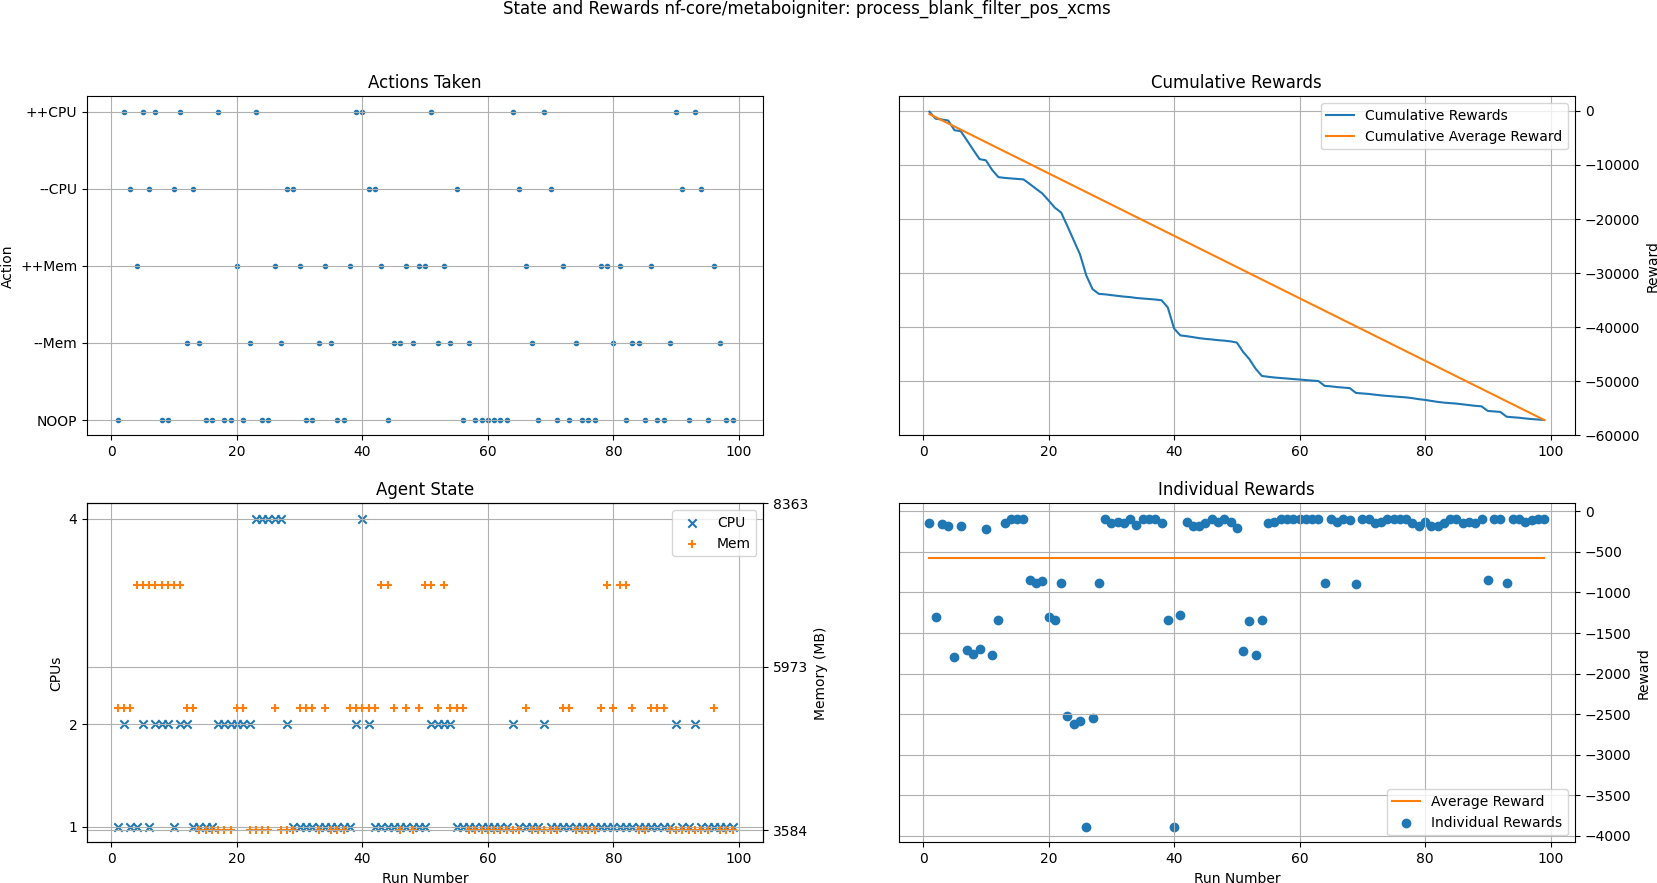
\includegraphics[width=\textwidth]{fig/qagent_cropped.png}
	\caption{Example of a Q-learning Agent}
	\label{fig:q_example}
\end{figure}

There are 4 graphs in \ref{fig:q_example} the top left graph is a scatter plot which indicates what action the agent took at what point in time. The bottom left graph indicates what the agent’s CPU and memory allocation (its state) was at that point in time. Meanwhile the top right graph shows the agent’s cumulative rewards over time, as well as a straight line which represents what the cumulative reward would look like if the reward was consistent. It should be noted that because the reward function is negative, whenever the line’s slope is steep the agent is performing poorly and receiving low rewards, whilst near-horizontal slopes show that the agent is doing well and limiting its punishment (receiving higher rewards). Finally the bottom right graph is a simple scatter plot of what rewards the agent received, with a constant line to show the average reward.

This figure is useful both to indicate that the agent is actually trying to learn favourable actions, as well as to represent what states the agent is exploring. 
